\section{Demoras por mes y distancia}

Se decidió analizar cómo se relacionan las demoras y la distancia del vuelo. Estas demoras tienen distintas causas, por lo que se prestó atención solamente a los siguientes tipos:
\begin{itemize}
\item Aerolínea (problemas de mantención del avión, o de los empleados)
\item Mal clima
\item NAS(National Aviation System, demoras causadas por operaciones del aeropuerto, tráfico voluminoso y/o control del tráfico aéreo)
\item Avión retrasado (demora por un vuelo anterior llegando tarde, causando que el vuelo presente salga más tarde)
\item Seguridad
\end{itemize}

\subsection{Primeras hipótesis y bases del análisis}

La hipótesis que se planteó respecto a este eje es que las causas de demoras afectan a los tipos de vuelo por igual, ya que las causas anteriormente nombradas no parecerían tener algún tipo de relación con la distancia del vuelo.

Para estos experimentos se utilizaron los datos entre los años 2003-2008 debido a que no se obtuvo información para años previos.

La figura 4 muestra la cantidad de vuelos por tipo, en la cual se observa que tanto los de corta, como mediana y larga distancia tienen una frecuencia similar y que escalan muy parecido en el tiempo.

%-Grafico 1
\begin{figure}[!htb]
\begin{center}
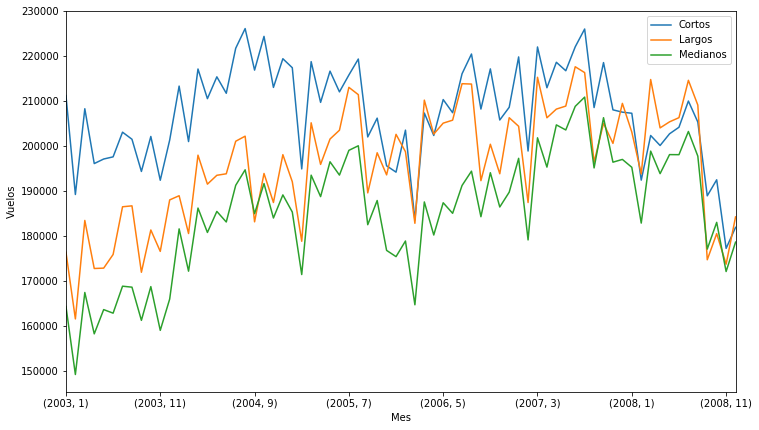
\includegraphics[scale=0.7]{distancia1.png}
\caption{Cantidad de vuelos por distancia}
\label{distancia-1}
\end{center}
\end{figure}

En la figura 5 se notó, primero que el porcentaje es muy similar para las 3 categorías. Hay menos retrasos en vuelos cortos, posiblemente debido a que necesitan una menor preparación, aunque no es una diferencia significativa. Otro dato que se extrajo de este gráfico es que las demoras son estacionarias, y tienen una frecuencia bastante regular ya que puede notarse que los altibajos se producen en las mismas épocas del año para los distintos tipos. Por esto se presta atención al estimar a los senos y cosenos.

% -Grafico 2
\begin{figure}[!htb]
\begin{center}
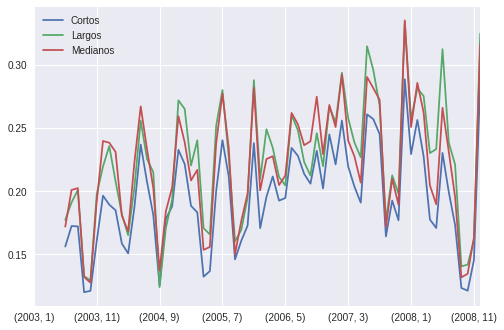
\includegraphics[scale=0.7]{distancia2.png}
\caption{Porcentaje de vuelos demorados por distancia}
\label{distancia-2}
\end{center}
\end{figure}



\subsection{Datos concretos y estimaciones}

Siguiendo el approach anterior, se estimó el porcentaje de demoras para vuelos medianos, tratando de estimar 2006, 2007 y 2008. Para cada año se tomó los dos años anteriores.

%Grafico 3 y 4
\begin{figure}[!htb]
\begin{center}
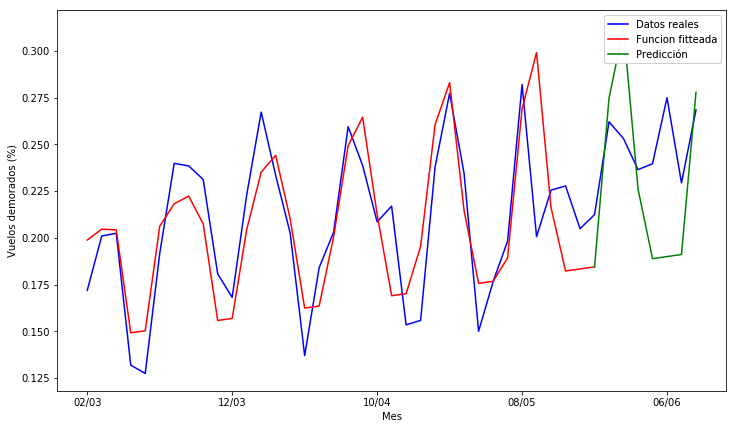
\includegraphics[scale=0.5]{distancia3.png}
\caption{caption}
\label{distancia-3}
\end{center}
\end{figure}

\begin{figure}[!hbt]
\begin{center}
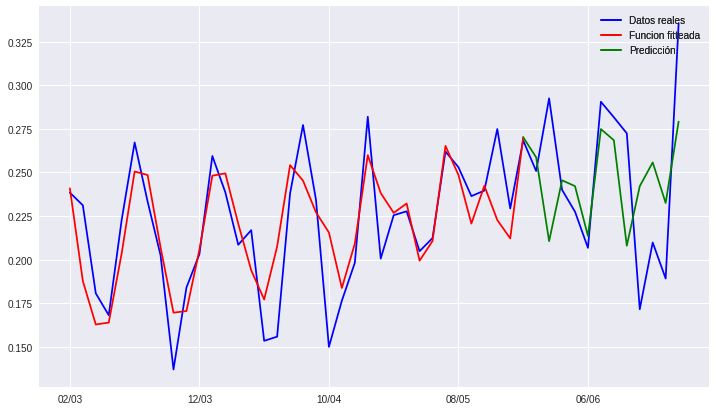
\includegraphics[scale=0.5]{distancia4.png}
\caption{caption}
\label{distancia-4}
\end{center}
\end{figure}

Los errores cuadráticos medios para estas estimaciones fueron 0.001143 (izquierda), y 0.001758 (derecha). La función utilizada con CML para esta estimación fue:

$f(x) = a + bx + c \times cos(xd + e) + f \times sin(xg + h) + i$

La intuición que se tuvo para encontrar la función fue usar cosenos y senos por la frecuencia y amplitud de los datos.

El experimento que se grafica en la figura 8 consistió en reutilizar los parámetros obtenidos por el método en el tipo de vuelo anterior y tratar de estimar el porcentaje de demoras para vuelos largos.

%Grafico 5
\begin{figure}[!htb]
\begin{center}
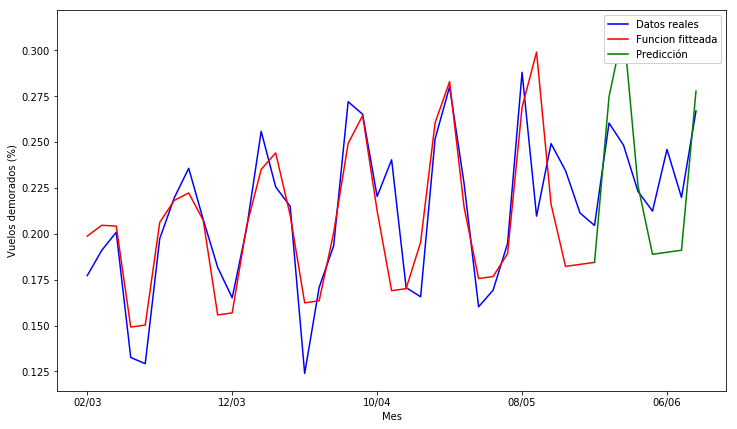
\includegraphics[scale=0.5]{distancia5.png}
\caption{caption}
\label{distancia-5}
\end{center}
\end{figure}

Como se puede observar la predicción se comporta bastante parecida a los datos reales, esta se acopla muy bien a la frecuencia, pero en el 2007 se puede observar una amplitud de los datos más pequeña que los años anteriores y ahí es donde más falló la estimación.